\documentclass[10pt,a4paper]{article}
\usepackage[utf8]{inputenc}
\usepackage[english]{babel}
\usepackage[square, numbers, sort&compress]{natbib}
\usepackage{graphicx}
\usepackage{float}
\usepackage{amsmath}
\usepackage{amsfonts}
\usepackage{amssymb}
%\usepackage{media9}
\usepackage{color}
\usepackage{fancyhdr}
\usepackage{lastpage}	
\usepackage{parskip}
\usepackage[scaled]{helvet}
\usepackage{blindtext}
\usepackage{sectsty}
\usepackage{multicol}
\usepackage{enumitem}
%\usepackage[svgnames]{xcolor}
\usepackage[labelfont={color=LibrelloColor,bf}, labelsep=period]{caption}
\renewcommand*{\familydefault}{\sfdefault}
\usepackage[left=1.75cm,right=1.75cm,top=1.75cm,bottom=3.75cm]{geometry}
\usepackage{titlesec}
\usepackage{svg}
\usepackage{flushend}
\PassOptionsToPackage{normalem}{ulem}
\usepackage{ulem}
	\providecolor{added}{rgb}{0,0,1}
	\providecolor{deleted}{rgb}{1,0,0}
	%% Change tracking with ulem
	\newcommand{\added}[1]{{\color{added}{}#1}}
	\newcommand{\deleted}[1]{{\color{deleted}\sout{#1}}}
\usepackage{setspace}
\usepackage[hyphens]{url}

% Green - CiS, OF
\definecolor{LibrelloColor}{RGB}{0,85,0}
% Red - JoHS
%\definecolor{LibrelloColor}{RGB}{128,0,0}



\usepackage[hidelinks, urlcolor=LibrelloColor]{hyperref}
\urlstyle{same}
\raggedcolumns
\flushcolumns
\usepackage{etoolbox}
%\usepackage{caption}
\usepackage{supertabular}
\usepackage{booktabs}
\usepackage{microtype}
\usepackage{threeparttable}
\usepackage{doi}
\usepackage{balance}
\usepackage{enumitem}
\usepackage{eurosym}
\usepackage{epstopdf}

\usepackage[color=yellow,icon=Comment,hoffset=-10mm, author=Librello Editorial's Office]{pdfcomment}

\titleformat{\section}
{\color{LibrelloColor}\normalfont\bfseries\filright}
{\color{LibrelloColor}\thesection.}{0.5em}{}

\titleformat{\subsection}
{\color{LibrelloColor}\normalfont\itshape\filright}
{\color{LibrelloColor}\thesubsection.}{0.5em}{}

\titleformat{\subsubsection}
{\color{LibrelloColor}\normalfont\itshape\filright}
{\color{LibrelloColor}\thesubsubsection.}{0.5em}{}

\usepackage{array} %criando coluna de largura fixa alinhada a esquerda
\newcolumntype{L}[1]{>{\raggedright\let\newline\\\arraybackslash\hspace{0pt}}p{#1}}
%criando coluna de largura fixa alinhada a direita
\newcolumntype{R}[1]{>{\raggedleft\let\newline\\\arraybackslash\hspace{0pt}}p{#1}}
\renewcommand{\arraystretch}{1.3}
\titlespacing\section{0pt}{12pt}{12pt}
\titlespacing\subsection{0pt}{12pt}{12pt}
\titlespacing\subsection{0pt}{12pt}{12pt}	
\renewcommand*{\refname}{References and Notes}

\fancypagestyle{document}{
	\renewcommand{\footrulewidth}{0pt}
	\renewcommand{\headrulewidth}{0pt}
	\renewcommand{\footrulewidth}{0pt}
	\renewcommand{\headrulewidth}{0pt}
	\renewcommand{\footskip}{40pt}
	\cfoot{\normalfont\thepage}
	\rhead{}\lhead{}
}

\fancypagestyle{firstpage}{
	\renewcommand{\footrulewidth}{0pt}
	\renewcommand{\headrulewidth}{0pt}
	\renewcommand{\footrulewidth}{0pt}
	\renewcommand{\headrulewidth}{0pt}
	\renewcommand{\footskip}{70pt}
	%CiS
	\lhead{Challenges in Sustainability $\mid$ 2017 $\mid$ Volume 5 $\mid$ Issue 1 $\mid$ Pages \thepage--\pageref{LastPage} \\DOI: 10.12924/cis2017.05010015\\
	ISSN: 2297--6477}
	\rhead{\includegraphics[height=0.59in]{CiS.eps}}
	%JoHS
%	\lhead{Journal of Human Security $\mid$ 2016 $\mid$ Volume 12 $\mid$ Issue 1 $\mid$ Pages \thepage--\pageref{LastPage} \\DOI: 10.12924/johs2016.12010112\\
%	ISSN: 1835--3800}
%	\rhead{\includegraphics[height=0.59in]{JoHS.eps}}
	%OF
%	\lhead{Organic Farming $\mid$ 2016 $\mid$ Volume 2 $\mid$ Issue 1 $\mid$ Pages \thepage--\pageref{LastPage} \\DOI: 10.12924/of2016.02010023\\
%	ISSN: 2297--6485}
%	\rhead{\includegraphics[height=0.59in]{OF.eps}}	
	\lfoot{\footnotesize © 2017 by the authors; licensee Librello, Switzerland. This open access article was published\\ under a Creative Commons Attribution License (\url{http://creativecommons.org/licenses/by/4.0/}).}
	\cfoot{}
	\rfoot{\vspace*{-24pt}\includegraphics[height=0.49in]{librello.eps}}

}

\makeatletter
\def\NAT@def@citea{\def\@citea{\NAT@separator}}
\makeatother

\begin{document}
\flushcolumns
\raggedcolumns



\pagestyle{document}
\thispagestyle{firstpage}


\vspace*{70pt}

\setlength{\parindent}{0cm}
\textit{Research Article}
%\textit{Review}
\vspace*{-12pt}

\begin{center}
\line(1,0){500}
\end{center}

\vspace*{12pt}
\begin{flushleft}
\begin{LARGE}
\textbf{{\color{LibrelloColor} Enabling Transformative Research: Lessons from the Eastern and Southern Africa Partnership Programme (1999--2015)}}\\
\end{LARGE}

\vspace*{12pt}

Cordula Ott

\vspace*{6pt}

Centre for Development and Environment, University of Bern, Bern, Switzerland. E-Mail: cordula.ott@cde.unibe.ch; \\Tel.: +41 316318822; Fax	: +41 316318544

\vspace*{6pt}

%* Corresponding author: E-Mail: Cmr138@txstate.edu; Tel.: +1 4794458334 
%
%\vspace*{15pt}

Submitted: 22 March 2016 $\mid$ In revised form: 3 October 2016 $\mid$ Accepted: 6 October 2016 $\mid$\\
Published: 27 February 2017
\end{flushleft}
\setcounter{page}{15}


\vspace*{-18pt}
\begin{center}
\line(1,0){500}
\end{center}

\vspace*{12pt}
%\vspace{\baselineskip}

\begingroup\leftskip= 1cm\rightskip 1cm  

\textbf{{\color{LibrelloColor}Abstract:}} World leaders at the 2015 United Nations Sustainable Development Summit in New York have reconfirmed the relevance of sustainability as the guiding paradigm in countering the development and climate crisis of the Anthropocene. Recent decades however, have been characterized by confusion, contestations, and arbitrariness in defining the nature and pathways of sustainable development. Humanity must urgently find ways to unlock the potential of the sustainability paradigm and organize a sustainability transformation. An emerging sustainability science community has already established considerable consensus on essential features of transformative science and research. Sustainability scholars are providing growing evidence that an emancipatory and democratic construction of sustainable development and more equitable, deliberative, and democratized knowledge generation are pivotal in tackling sustainability challenges. These findings are further underpinned by experiences gained in the \textit{Eastern and Southern Africa Partnership Programme} (1999--2015)---a rare case of a long-term, transnational, and transdisciplinary research endeavour already completed. The programme fulfilled the dual role which is compulsory in transformative research: It generated contextualized knowledge and innovation at the science–society interface while simultaneously securing meaningful participation and Southern agency in a co-evolutionary process. This paper offers insight into the programme’s adaptive structure and implementation processes, which fostered deliberation, capacity development, and joint programme navigation benchmarked against local needs and broader sustainability demands. The ESAPP experience confirms that, if taken as the overarching frame of reference for all actors involved, the sustainability paradigm unfolds its integrative and transformative power. It enables sustainability-oriented actors from all scientific and practical fields to seek consilience between differing development and innovation paradigms and synchronize their development agendas and research frameworks on behalf of societal co-production of knowledge and innovation. Accordingly, the sustainability paradigm has the power to guide development and innovation policy, and practice out of the current confusion and ineffectiveness. 

\textbf{{\color{LibrelloColor}Keywords:}} capacity development; deliberation; equity; innovation; knowledge; partnerships; research; sustainability science; sustainable development; transformation
\par\endgroup
 
\setlength{\parindent}{0.5cm}
\setlength{\parskip}{0cm}
\setlength{\bibsep}{0cm}

\vspace*{10mm}
%\vspace*{20mm}

\begin{multicols}{2}

\section{Introduction}
\subsection{Confusion and Arbitrariness in the Understanding of Sustainable Development}
\noindent At the 2015 United Nations Sustainable Development Summit in New York, world leaders responded to alarming scientific evidence showing that we humans are interfering with the Earth system at a scale and magnitude that threatens our own survival. With the adoption of the \textit{2030 Agenda for Sustainable Development and its 17 Sustainable Development Goals} (SDGs), they reconfirmed the primacy of sustainability as the guiding development paradigm (UN, 2015). Framed in the so-called ``Brundtland Report'' \citep{r01} and endorsed at the 1992 Earth Summit in Rio, the sustainability paradigm is not novel; and looking back, it has fallen short of expectations in various ways. Nevertheless it continues to be the official global response to the development and climate crisis of the Anthropocene. But---and this is confirmed by the renewed global commitment---science and society must urgently find ways to unlock its potential and organize a sustainability transformation \citep{r02}.

The Post-Brundtland world is characterized by confusion, contestations, and arbitrariness in identifying the nature and pathways of sustainable development \citep{r03, r04, r05}. The implications of the sustainability paradigm as an antithesis to the paradigm of growth and transfer are not easy to capture. Although our understanding of development intervention and global governance has fundamentally changed \citep{r06, r07, r08}, the normativity and the transformative power of sustainability have reached buzzword status \citep{r09}. At the same time, unorthodox scholars across diverse fields in science, technology, and development, have observed narrow, exploitative, and often destructive use of promising post-Rio development concepts such as innovation \citep{r10, r11}, gender mainstreaming \citep{r12}, livelihoods \citep{r13, r14}, justice \citep{r15}, or transformation \citep{r16}, to mention just a few. Scholars argue that systemic thinking, equity-based science-society interaction, and reflexive learning – which are all indispensable in generating knowledge and innovation for sustainable development---continue to be marginalized, confined to single sectors, and used to serve vested interests \citep{r17, r18, r19}. Despite progress on the integration of civil society in global environmental assessments and negotiations, power disparities and self-interest are hampering action and creating new tensions, disparities, and bargaining between the global North and South \citep{r20, r21, r22, r23}. While economic bias gets much of the attention in the debate, sustainability scholars also criticize frequent environmental bias at the expense of human and social issues \citep{r04}, and social bias. The latter prevailed in the Millennium Development Goals, for example \citep{r24}. Spangenberg (\citep{r18} p. 277) points out a damaging ``trend towards a further fragmentation of research concerning the substance of sustainability''. Skoglund and Jensen (\citep{r22} p. 124) provide a striking example of how climate policy is misguided; they refer to Chandler (2012), who showed ``how different policies and non-governmental organizations rely on the `adaptation agenda' to suggest survival strategies for the poor: thus attempting to align the marginalized with `vulnerability to climate change', instead of addressing the broader economic and social factors that gave rise to their marginalized position''. Such examples illustrate how concrete efforts and successes fade in an amalgam of overlapping and often contradictory approaches and discourses ranging from mainstream sustainability to green radicalism \citep{r25}, or from weak sustainability to more radical constructions of strong sustainability \citep{r04, r26, r27}. As a consequence, the pre-Brundtland paradigm of growth, with its ``loading-dock approach'' \citep{r28} of transferring scientific and technological solutions to decision-makers, is persisting \citep{r29, r30}. To break its dominance and unlock transformative potentials, sustainability advocates have begun to reclaim the emancipatory power inherent in the original conceptualizations of development in their respective disciplines and practical domains. Taking systems approaches, they strive for epistemological and practical grounding as well as for further clarification of the interfaces between diverse development concepts (see, for example, \citep{r09, r10, r11, r19, r31, r32, r33, r34}). 

This leads to the approach I take in this paper. My overarching question is: How can science contribute to a sustainability transformation? More specifically, I reflect on various aspects that are essential in organizing transformative research. I argue that an emancipatory and democratic construction of sustainable development is pivotal in tackling sustainability challenges. An emerging sustainability science is providing growing evidence of this fact. I further underpin my argument with experiences gained in the \textit{Eastern and Southern Africa Partnership Programme}---a rare case of a long-term transdisciplinary research endeavour already completed. With my contribution, I intend to confirm that, if taken as the principal frame of reference, sustainable development is suited to integrate the efforts of sustainability-oriented scholars and practitioners across different profiles. It provides orientation in synchronizing development agendas and frameworks towards societal co-production of knowledge and innovation. Accordingly, the sustainability paradigm has the power to guide development and innovation policy and practice out of the current confusion and ineffectiveness. 

\subsection{An Emancipatory Construction of Sustainable Development}
\noindent Fortunately, we can build on promising achievements in transformative research. A multitude of reviews and syntheses show how an emerging sustainability science community is establishing considerable consensus on the sustainability paradigm's epistemological and practical implications for science and research (see, for example, \citep{r08, r16, r18, r22, r27, r29, r35}). With a view to promoting equity-based, just development within the planetary boundaries, scholars are working to identify enabling institutional contexts and developing transdisciplinary research frameworks and procedures across scientific disciplines and at the interfaces between science and society, as well as between science and policy \citep{r32, r36, r37, r38, r39, r40}. They conceive of sustainability as a societal future forming process \citep{r05}, as it ``emerges as a horizon to be approached but never reached'' (\citep{r42} p. 992). Accordingly, transdisciplinary theory and practice must accommodate pluralism and experimentation. But, as Waas and colleagues (\citep{r04} p. 1645) point out, this future forming process has to be benchmarked against the ``precise and unambiguous meaning'' of the original conceptualization of sustainable development. They identify four fundamental principles---normativity, equity, integration, and dynamism---that ``represent the interpretational limits of the concept and are essential to sustainability no matter which view and interpretation is employed'' (\citep{r04} p. 1657). Such (and analogous) principles respond to the complexity and adaptiveness of human–environment systems---which are the subject under consideration \citep{r33, r43}---and provide orientation for societal future forming processes and ``research in a world of flux'' (\citep{r05} p. 11). Ethical and equity concerns further underpin sustainable development as an emancipatory and transformative concept and open the floor for contesting existing power structures and decision-making processes \citep{r16, r26, r44}. Not only natural resources but also social capital and knowledge must be distributed equally \citep{r23, r45, r46, r47}. This requires us to rethink our understanding of knowledge and expertise, and to revise our traditional role and (self-)conception as researchers \citep{r41, r48, r49}. Normative, democratic and procedural principles are at the core of transdisciplinary practice, in which scholars attempt to link science and civil society in joint reflexive or learning processes \citep{r17, r18, r26, r38, r40}. Building on such critical reflection, sustainability scholars are bringing together long-standing participatory, democratic, and social movements' traditions and structuring research along new, deliberate forms of science–society interaction \citep{r51, r52, r53, r54}. In a deliberative democracy, or indeed in any deliberative system, actors participate in a communicative process and influence collective decisions \citep{r25, r55}. If we understand a research framework or programme as a deliberative system, its deliberative capacity---``the extent to which a political system possesses structures to host deliberation that is authentic, inclusive, and consequential'' \citep{r51}---gains utmost importance. But the deliberative capacity of individuals and institutions involved must likewise be secured for their equal and meaningful inclusion in future forming processes.  As well as putting equity and power issues to the fore, this undergirds the strategic goal framed by the United Nations Educational, Scientific and Cultural Organization to develop knowledge societies by democratizing knowledge and knowledge generation \citep{r56}. Indeed, progress in the democratization of knowledge has been observed \citep{r57}, and sustainability science is making headway. But transdisciplinarity is a relatively young field, and experiences of long-term transdisciplinary practice at a transnational, regional scale are particularly rare.

In the following, I will present the \textit{Eastern and Southern Africa Partnership Programme} (ESAPP) as a research endeavour that is well-suited to help fill this gap. Running from 1999 to 2015, the programme brought together partners from Switzerland, Kenya, Ethiopia, Tanzania, Madagascar, Mozambique, and Eritrea in conducting long-term transdisciplinary research for sustainable land management and sustainable regional development. Two final publications provide substantial insights into this experience. Ehrensperger and colleagues present ESAPP's research and outcomes \citep{r58}, while Ott and Kiteme \citep{r59} provide more in-depth reflections on the implementation, adaptation, and learning processes that took place within ESAPP. Taking up the arguments outlined above, I present programme features that proved to be supportive in strengthening deliberative capacity, equity-based knowledge generation, and institutional development for coherent local to global governance. I further discuss specific challenges that arose during the implementation of this transdisciplinary and transnational research programme as well as in securing its legacy.

\section{Cornerstones of Transformative Research in the Eastern and Southern Africa Partnership Programme}

	
\subsection{An Enabling Institutional Context}
\noindent \textls[-5]{When ESAPP was framed in the late 1990s, both public involvement and sustainability science were in their infancy. Ott and Kiteme \citep{r59} show how three contextual developments at the interface between science and policymaking had prepared the ground for ESAPP's unique and innovative programme design: First, decades of research collaborations and networking between Switzerland and countries in Eastern Africa had established trust and fruitful interaction between scientists, funding organizations, as well as governmental and non-governmental actors and institutions of the countries involved. This led to the launching of an integrative research programme that matched the scientific and political landscape of Eastern Africa. Second, since 1988, ESAPP's mother institution, the University of Bern's \textit{Centre for Development and Environment }(CDE), had been mandated by the \textit{Swiss Agency for Development and Cooperation} (SDC) to help prepare Switzerland's position on the 1992 Rio conventions and translate them into poverty alleviation policy and practice. Already in the 1990s, CDE had come up with integrative, participatory concepts and tools designed to support human agency, science–society interaction, and social learning \citep{r60}. Third, the programme designers could build on long-standing activities of a loose network of sustainability-oriented scholars and practitioners in Switzerland. In 1997, representatives from CDE and the Swiss Academy of Sciences and its \textit{Commission for Research Partnerships with Developing Countries} (KFPE) drafted the KFPE's 11 Principles and 7 Questions as a guide for transdisciplinary and transnational research partnerships for sustainable development \citep{r45, r61}. The KFPE guide is heavily equity-oriented and reflects state-of-the-art sustainability science even today. It underpins the choice of sustainable development, partnership, and transdisciplinarity as ESAPP's core foundations. The well-established collaboration between scientists, practitioners, and policymakers enabled SDC as the funding institution to give ESAPP's architects considerable leeway; at the same time, SDC was represented on ESAPP's advisory board---the programme's steering committee---from the outset. Such long-standing and trustful collaboration between researchers, funding organisations, and research users in the North and South, must be considered a precondition for transformative research \citep{r59}.}

\subsection{Emancipatory Foundations: Sustainable Development, Transdisciplinarity, and Partnership}
\noindent ESAPP was launched in 1999 with the mission of generating new knowledge and innovation for sustainable development on local to regional levels. The programme was aimed at mitigating sustainability challenges by making knowledge generation more democratic and accessible, increasing Southern ownership and agency, producing innovative research results, and promoting evidence-based, South-driven sustainable rural development. Transdisciplinarity as the second epistemological pillar of ESAPP was understood as an integrative approach that brings together scientific (disciplinary and interdisciplinary) and non-scientific (endogenous, indigenous, cultural, local, etc.) knowledge systems; academic, social, and political actors and institutions; and different places and scales \citep{r50, r52}. This approach would guide science and society through research and learning processes in which they needed to jointly produce three types of knowledge: systems knowledge, which delineates the sustainability problem to be addressed and the associated subsystem or context (``What is?''); target knowledge, which encompasses negotiated values and goals for a shared vision of a sustainable future (``What ought to be?''); and transformation knowledge, which describes the path to follow in order to achieve a sustainable future (``How do we get there?'') \citep{r39, r53, r61}. In such an understanding, knowledge and innovation for sustainable development are necessarily an outcome of joint learning processes that involve all societal actors. Accordingly, ESAPP framed research for sustainable development as what Gergen \citep{r05} has called a future forming practice. The programme constituted itself as a communicative space \citep{r55, r62} embedded in an open framework of research partnerships. ESAPP's developers further acknowledged that partnership as a third epistemological pillar required special attention. In North–South research partnerships, disparities with regard to power, knowledge, and resources often constrain balanced exchange and cooperation, as the research is generally financed, initiated, managed, and evaluated by Northern institutions \citep{r67}. In a network as complex as ESAPP's, this calls for efforts to expand deliberative capacity, for a devolution of power, and for ensuring accountability and legitimacy towards both funding organizations and partners within and beyond the research network \citep{r08, r39}. It requires management strategies and organizational structures that promote Southern partners' determination, competence, and ownership with respect to the formulation of pathways to sustainable development \citep{r44, r57}. And this, in turn, calls for pragmatism \citep{r03, r63}. Pursuing equity as a structural goal within ESAPP was both fundamental and innovative.

\textls[-10]{Another central conceptual element in ESAPP was its thematic and spatial concentration. In line with CDE’s core competence, ESAPP focused on contextualized knowledge about sustainable land management and sustainable regional development and promoted local and regional initiatives through transdisciplinary research. Knowledge has to be generated and processed together with local actors to be robustly coupled to human-environment-system dynamics in a specific context \citep{r33, r63, r64}. In the African context, a vast majority of people depend on direct access to renewable natural resources, while competing claims and short-term needs at various scales tend to override environmental concerns, aggravate poverty, and inhibit economic development \citep{r65}. The result is a dwindling resource base, which often goes unnoticed for a long time. The programme’s stewardship of the environment does not constitute a case of the environmental bias observed by Waas and colleagues \citep{r04}; it is a necessity. After many decades of neglect, rural areas and the livelihoods of small-scale resource users are now being reappraised based on the recognition that global governance approaches, adaptation and mitigation strategies must build on knowledge of local conditions to be effective \citep{r21, r66}.}

\subsection{Adaptive Research Structures}
\noindent ESAPP’s designers were well aware that the programme's transdisciplinary and transnational research framework opened up a door to many new challenges. One of these challenges is the dual role of scientists doing transformative research: they must work to provide evidence while simultaneously expanding human and institutional capacity for sustainable development by means of education and training, collaborative research and learning processes, as well as knowledge brokering activities and products \citep{r30, r51, r54, r67}. How then should inter- and transdisciplinary research be (re-)organized and structured? A sophisticated research framework is provided by the Earth System Governance Project, which organizes research around five analytical problems: architecture, agency, adaptiveness, accountability, and allocation \& access. At the same time power, knowledge, norms, and scale are regarded as crosscutting research themes that are crucial to the study of each analytical problem and also to an integrated understanding of earth system governance. Related thematic issues are embedded in flagship activities \citep{r37}. This research framework outlines, in a very useful way, the basic challenge of coherently integrating facts and values in a transdisciplinary research programme \citep{r37, r41}. In ESAPP, conceptual and operational challenges or necessary trade-offs at the science–policy interface were addressed by combining the open partnership and research framework with recursive and (self-)reflexive processes that the project partners steered jointly \citep{r39}. Three structural approaches provided the necessary guidance (see also \citep{r59}):

\begin{enumerate}
\item \textit{An adaptive management approach that integrates actors' agency}: Adaptive management corresponds well with a recursive and reflexive research design. Widely accepted today, adaptive management of a research programme was innovative at the turn of the millennium. ESAPP’s adaptive management approach was intended to provide the necessary basic stability in the institutional fabric while allowing for goals, institutional structures, and research procedures to be reshaped in the course of the programme’s implementation. It offered space for integrating feedback and research results into management decisions and securing meaningful participation and institutional development. 
\item \textit{A dual-structure approach that harmonizes concepts and action}: In development contexts, short-term priorities often override long-term sustainability imperatives. This may result in a one-sided focus on either basic research or action research, or in the latter being viewed as a mere add-on to business-as-usual science. To accommodate both need-driven and concept-driven concerns, ESAPP linked action research with basic research and capacity development. The two components were intended to interact, reinforce each other, and eventually reshape the programme. ESAPP’s action research component comprised over 300 small-grant priority action projects formulated by local partners alone or in collaboration with ESAPP researchers. The basic research and capacity development component mainly served to provide support and secure programme coherence, consistency, and effectiveness through reflection, learning, and adaptation.
\item \textit{A contextuality approach that links places and scales}: At its outset, ESAPP was mandated to build on contextualized knowledge, databases, capacities and partner networks created by CDE's predecessor programmes in Africa; to further develop their transdisciplinary character; and to make them available for decision-making support and further research. Knowledge and data for sustainable land management and sustainable regional development that are contextualized---embedded in a specific time, place, and scale---are currently high on the global development agenda. Building and consolidating bottom-up databases and linking them with regional or global observatories is critical to enhancing coherence and consistency in governance approaches from local to global levels. In addition, it is a key asset for developing countries in formulating self-determined and just national development strategies and in interacting with global development institutions \citep{r30, r64}. 
\end{enumerate}

Being at once consistent, integrative, and flexible, ESAPP's three structural approaches secured an institutional arrangement that was ideally suited for enhancing deliberative capacity, learning, and institutional development. In what follows, I will provide some insight into how indeed, they fostered equity and inclusion, the co-production of contextualized knowledge, and the development of people's and institutions' capacities, in the South and North (see also \citep{r59}).

\subsection{Joint Programme Navigation for Sustainable Development}
\noindent As argued above, in order to support a sustainability transformation, scientists need to strengthen the deliberative capacity of research--- understood as a political system---by means of adequate structures and procedures. Adequacy in this context means that they are in line with the fundamental normative, democratic and procedural principles of sustainable development. It is in collaborative and reflexive processes that partners in research share and integrate values, norms, and perceptions, tackle dissent, and create a ``common culture''. This shifts the focus from research outcomes to the processes of social knowledge generation; to experimentation, learning, and constant change under an adaptive governance approach \citep{r30, r54, r62}. The ``communicative space''---actual or virtual meeting places---and the deliberate and consequential quality of exchange become a subject of analysis: Where do researchers, partners, and actors interact, and what exactly are they doing there? But first of all, people need to be brought together. For the ESAPP as a transnational research programme, this was not only a logistical problem. Organizing joint processes among partners with different cultural backgrounds and varying institutional strength requires time, resources, and mutual trust. Over the years, ESAPP partners successfully organized an iterative process of reflection and adaptation within routine modes and places of exchange. The following elements and milestones of partners' interaction were crucial to this success: 

\begin{itemize}
\item \textit{Institutionalizing joint programme steering}: Like many endeavours in the field of research for development, ESAPP was North-funded and hence North-driven at its inception. The advisory board---the programme's steering body---was composed by representatives of SDC as the funding institution, of CDE, and of related Swiss institutions. Southern partners were not represented until 2011. But early assessments emphasized the need for strengthening Southern partners' capacity and ownership to increase equity and ensure research coherence, relevance, and quality for the benefit of the South. Eventually, in 2006, partners initiated annual one-week capitalization workshops in the South to overcome geographic distance, foster communication, and exchange on a regular base. The workshops immediately became the cornerstone of joint programme management. Here, ESAPP partners met for data and method sharing, deliberation and self-evaluation, strategic reorientation, and a field excursion. Here, they applied and further developed ESAPP's management tools, settled conflictive issues, and made necessary changes in the programme's organizational structure and research design.
\item \textit{Developing adequate management tools and procedures}: Of necessity and custom, at the outset of the programme, criteria for selecting research projects, as well as monitoring and evaluation mechanisms mainly reflected goals and indicators valued in the North. In the course of time, partners jointly identified new forms of process benchmarking: They developed an appropriate monitoring and evaluation system that combined reflexive elements (self-evaluation, feedback loops) with simple and easy-to-understand standard formats (project documents, catalogues of criteria, target matrices/log frames, statistical evaluations, etc.) and standard procedures (advisory board meetings, project-cycle steps, external evaluations, etc.). Being fairly consistent, lean, and procedural, ESAPP's monitoring and evaluation system served as a navigation tool \citep{r45}.
\item \textls[-5]{\textit{Scaling research results up and out}: Given the high pressure for quick and effective interventions in rural development contexts, ESAPP was confronted with high numbers of priority action project proposals. To secure ESAPP's mission and scope, the partners established a process of clustering and sequencing thematically related projects. A preselection of projects was done by the coordinators in the respective partner countries. In the annual capitalization workshops, projects were further discussed, evaluated, and related to one another. Eventually, this led to the creation of thematic partnerships between countries which promoted the scaling up and out of results within the whole region. Finally, ESAPP consolidated its research in ten reference sites characterized by context-specific priorities within the region. This procedural thematic concentration made it possible to use research results of more than 300 priority action projects as evidence in an ``ongoing process of evaluation, learning, adaptation and adoption'' (\citep{r62} p. 492).}
\item \textit{Consolidating and leveraging ESAPP's knowledge and database}: Partners jointly upgraded and made available a comprehensive long-term database that includes geo-referenced long-term measurements and observations of natural resources that  links ecological and socio-economic quantitative and qualitative knowledge at local, national, and regional levels. It is a key asset for research and policymaking in Eastern Africa and the backbone of ESAPP's Southern network. At the same time, the database is a major tool for education and capacity development beyond the programme's lifetime that led to the generation of local knowledge platforms and institutions. The knowledge database also includes a set of transdisciplinary tools. Tools that combine analytical and communicative elements---that is, tools that merge empirical research with participatory assessments and social learning---proved especially successful.
\item \textit{Consolidating and leveraging ESAPP's network of partners}: In the implementation and learning processes of ESAPP, partners jointly consolidated initially broad and loose networks. Southern institutions gradually became more equal partners within the programme. Partner institutions were not equally strong in all countries---indicating a need for better integration---but in some countries they were able to initiate new strategic collaborations and networks. The ESAPP network also includes hundreds of government officials, experts, and researchers that participated in ESAPP training courses, especially in those organized by the Centre for Training and Integrated Research in Arid and Semi-Arid Lands Development (CETRAD, Kenya). CETRAD itself is a major outcome of research collaboration between Switzerland and Kenya. The Water and Land Resource Centre (WLRC) in Ethiopia is another example. But many other institutions, down to the village level, grew out of ESAPP research activities. 
\end{itemize}

\section{Challenges and Outlook}
\noindent A sustainability transformation requires novel research frameworks and programme structures that accommodate processual and democratic features such as normativity, equity, integration, dynamism, inclusiveness, accountability, legitimacy, deliberation, and others \citep{r04, r25, r37}. The Eastern and Southern Africa Partnership Programme, ESAPP, was as an early transdisciplinary research endeavour that successfully endorsed inclusive, authentic, and consequential deliberation and joint programme navigation balancing local needs and sustainability demands. The programme thus fulfilled the dual role which is compulsory in transformative research: It generated contextualized knowledge and innovation at the science–society interface while at the same time securing meaningful participation and Southern agency in a co-evolutionary process \citep{r55, r68}. But despite ESAPP’s widely acknowledged success, the programme’s final assessments list major shortcomings \citep{r58, r59}. For example, research in the complex transnational and transcultural context of ESAPP was constrained considerably by standard planning and budget frameworks, which generally do not favour experimental procedures and equity approaches. Insufficient human and institutional capacities, a lack of ownership among the funding and collaborating institutions, and weak South–South engagement were other limiting factors. The jointly developed monitoring and evaluation system for guiding both action research projects and institutional development remained insufficiently coherent. Managing a comprehensive database and relating it to existing regional environmental databases and global observatories proved too ambitious and challenging for a research programme as small as ESAPP. In some countries, the number of action research projects was too small to enable meaningful clustering and scaling up of results. The programme's success in strengthening the Southern network and equitable South–South exchange was limited by differences in political and institutional backgrounds and by national interests overriding collaborative efforts. Although promising ways of tackling stumbling blocks and trade-offs at the interfaces between science, society, and policy are well-described \citep{r36, r39, r41} and were included in ESAPP's design, the programme's implementation was continuously contested by partners within and beyond the programme. Here, the sustainability paradigm unfolded its integrative and transformative power and helped to focus collaborative processes within the programme. Taken as a superordinate system of reference that is valid for all actors involved, it implied, and guided equity-based and democratic processes of research, learning, and innovation. A basic characteristic was that actors jointly identified research needs and approaches, and that they jointly assessed, evaluated, and reused evidence and innovations. 

Such reflexive and recursive processes are well-suited for integrating different development and innovation paradigms in a fruitful way, particularly the dominant \textit{innovation paradigm that takes science as its frame of reference}---that is, where scientists and researchers provide and transfer the ``right'' knowledge and solutions to decision-makers---and the fairly widespread \textit{innovation paradigm that builds on interaction between science and society}. Both paradigms have proved to be insufficient in themselves, but they can nonetheless be an important part of solutions for sustainable development. In ESAPP's final report \citep{r58}, partners provide many examples. But an important lesson learned during ESAPP is that the sustainability paradigm goes beyond the innovation paradigm building on science–society interaction. Born in the spirit of the 1980s, this innovation paradigm holds that scientists and civil society should communicate to improve the efficiency and effectiveness of development measures, enable evidence-based decision-making, and ensure an ethically sound application of knowledge. But this paradigm causes misunderstandings, resistance, and conflicts because actors in science, governmental and non-governmental institutions, business, and communities relate to different systems of reference. The concept of science–society interaction remains vague; criteria and measures of evidence and success depend on the different actors' negotiation power; and power disparities increase the commodification and economic evaluation of research \citep{r49}. By contrast, an innovation paradigm that takes sustainable development as its overarching emancipatory frame of reference---as applied in ESAPP---opens ways out of the confusion that characterizes the post-Brundtland world. It replaces unspecific interaction between science and society by integrating actors, knowledge, and value systems in joint learning processes, and supports the fundamentally novel understanding of knowledge and innovation applied in sustainability science. It enables sustainability-oriented actors from all scientific and practical fields to seek consilience \citep{r34}, and synchronize their development agendas and research frameworks on behalf of societal co-production of knowledge and innovation.

But transdisciplinary practice is inherently complex, resource-consuming, and often fails. We must bear in mind that in the complexity of future forming processes, or ``research in a world of flux'' (\citep{r05} p. 11), achievements – but also shortcomings---are always preliminary, procedural, and gradual. Nevertheless, transformative science is a necessary counterculture to today's technocratic focus on evidence and outputs. It requires long-term commitments, collaborations and partnerships, as well as strong leadership by visionary actors in science and practice. In light of ESAPP's experience, researchers, policymakers, and funding institutions would do well to conceive of North–South research partnerships as a long-term, co-evolutional process between countries and world regions. As Garud and Geman (\citep{r42} p. 992) put it, ``(\ldots) the challenge for policy, strategy and research is not just a matter of becoming sustainable, but of sustaining the ability to embark on such journeys on an ongoing basis''. If this journey ends when a programme is completed, the translation of transdisciplinarity into governance processes and institutions in partner countries in the global South will not endure. 

\section*{Acknowledgements}
\noindent This paper presents the author’s personal view. It was partially presented at a number of international sustainability fora, including the 2014 \textit{Norwich Conference on Earth System Governance: Access and Allocation in the Anthropocene}, held on July 1--3, 2014 in Norwich, UK; the \textit{Ethics of Poverty Alleviation Conference}, held on August 28--29, 2014 at the Centre for Ethics and Poverty Research, University of Salzburg, Austria; the 2015 Annual Conference of the European Forum on Studies of Policies for Research and Innovation (Eu-SPRI), on \textit{Innovation Policies for Economic and Social Transitions: Developing Strategies for Knowledge, Practices and Organizations}, held on June 10--12, 2015 in Helsinki, Finland; and the 2015 \textit{Canberra Conference on Earth System Governance: Democracy and Resilience in the Anthropocene}, held on December 14--16, 2015 in Canberra, Australia. I gratefully acknowledge the support of the Centre for Development and Environment (CDE) and all partners in the Eastern and Southern Africa Partnership Programme (ESAPP) and the valuable comments made by anonymous peer reviewers.

\end{multicols}
\clearpage

\vspace{\baselineskip}

\begin{multicols}{2}
\renewcommand*{\refname}{\normalsize{References and Notes}}

\begin{footnotesize}
%\bibliographystyle{vancouver_Librello}
%\bibliography{267-Biblio}

\begin{thebibliography}{10}

\bibitem{r01}
Our Common Future: The Report of the World Commission on Environment and
  Development.
\newblock Oxford, UK: Oxford University Press; 1987.

\bibitem{r02}
Back to Our Common Future: Sustainable Development in the 21st century (SD21)
  project, Summary for policymakers.
\newblock United Nations Department for Economic and Social Affairs (UN-DESA).

\bibitem{r03}
Sneddon C, Howarth RB, Norgaard RB.
\newblock Sustainable development in a post-Brundtland world.
\newblock Ecological Economics. 2006;57(2):253--268.
\newblock
  \href{https://doi.org/10.1016/j.ecolecon.2005.04.013}{doi:10.1016/j.ecolecon.2005.04.013}.

\bibitem{r04}
Waas T, Hug{\'{e}} J, Verbruggen A, Wright T.
\newblock Sustainable Development: A Bird's Eye View.
\newblock Sustainability. 2011;3(12):1637--1661.
\newblock \href{https://doi.org/10.3390/su3101637}{doi:10.3390/su3101637}.

\bibitem{r05}
Gergen KJ.
\newblock From Mirroring to World-Making: Research as Future Forming.
\newblock Journal for the Theory of Social Behaviour. 2014;45(3):287--310.
\newblock \href{https://doi.org/10.1111/jtsb.12075}{doi:10.1111/jtsb.12075}.

\bibitem{r06}
Kates RW, Clark WC, Corell R, Hall JM, Jaeger CC, Lowe I, et~al.
\newblock Sustainability Science.
\newblock Science. 2001;292(5517):641--642.
\newblock
  \href{https://doi.org/10.1126/science.1059386}{doi:10.1126/science.1059386}.

\bibitem{r07}
World in Transition---A Social Contract for Sustainability.
\newblock Berlin, Germany: German Advisory Council on Global Change (WBGU);
  2011. Flagship Report.
\newblock Available from:
  \url{http://www.wbgu.de/en/flagship-reports/fr-2011-a-social-contract/}.

\bibitem{r08}
Biermann F, Abbott K, Andresen S, Backstrand K, Bernstein S, Betsill MM, et~al.
\newblock Navigating the Anthropocene: Improving Earth System Governance.
\newblock Science. 2012;335(6074):1306--1307.
\newblock
  \href{https://doi.org/10.1126/science.1217255}{doi:10.1126/science.1217255}.

\bibitem{r09}
Santillo D.
\newblock Reclaiming the Definition of Sustainability.
\newblock Environmental Science and Pollution Research - International.
  2007;14(1):60--66.
\newblock
  \href{https://doi.org/10.1065/espr2007.01.375}{doi:10.1065/espr2007.01.375}.

\bibitem{r10}
Lundvall B.
\newblock The origins of the national innovation system concept and its
  usefulness in the era of the globalizing economy.
\newblock In: 13th Globelics Conference. Havana, Cuba; 23--26 September 2015.
  Available from:
  \url{http://www.globelicsacademy.net/Lundvall_NSI-origins%20and%20globalisation.pdf}.

\bibitem{r11}
Benneworth P, Amanatidou E, {Edwards Schachter} M, Gulbrandsen M.
\newblock Social innovation futures: Beyond policy panacea and conceptual
  ambiguity.
\newblock Oslo, Norway: University of Oslo; 2015. TIK Working Paper No.
  20150127.
\newblock Available from:
  \url{https://ideas.repec.org/p/tik/inowpp/20150127.html}.

\bibitem{r12}
Brody A.
\newblock Gender and Governance.
\newblock Institute of Development Studies, University of Sussex; 2009.
  Overview report.
\newblock Available from:
  \url{http://www.bridge.ids.ac.uk/reports/Governance_OR_final.pdf}.

\bibitem{r13}
Scoones I.
\newblock Livelihoods perspectives and rural development.
\newblock The Journal of Peasant Studies. 2009;36(1):171--196.
\newblock
  \href{https://doi.org/10.1080/03066150902820503}{doi:10.1080/03066150902820503}.

\bibitem{r14}
Wiesmann U, Ott C, {Ifejika Speranza} C, Kiteme BP, Müller-Böker U, Messerli
  P, et~al.
\newblock A human actor model as a conceptual orientation in interdisciplinary
  research for sustainable development.
\newblock In: Wiesmann U, Hurni H, editors. Research for Sustainable
  Development: Foundations, Experiences, and Perspectives. Perspectives of the
  Swiss National Centre of Competence in Research (NCCR) North-South. Bern,
  Switzerland: Geographica Bernensia; 2011. pp. 231--256.

\bibitem{r15}
Schlosberg D, Collins LB.
\newblock From environmental to climate justice: climate change and the
  discourse of environmental justice.
\newblock Wiley Interdisciplinary Reviews: Climate Change. 2014;5(3):359--374.
\newblock \href{https://doi.org/10.1002/wcc.275}{doi:10.1002/wcc.275}.

\bibitem{r16}
Patterson J, Schulz K, Vervoort J, Adler C, Hurlbert M, van~der Hel S, et~al.
\newblock `Transformations towards sustainability': Emerging approaches,
  critical reflections, and a research agenda.
\newblock Lund, Sweden: Lund University; 2015. Earth System Governance Working
  Paper No. 33.

\bibitem{r17}
Ulrich W.
\newblock Reflective Practice in the Civil Society: The contribution of
  critically systemic thinking.
\newblock Reflective Practice. 2000;1(2):247--268.
\newblock \href{https://doi.org/10.1080/713693151}{doi:10.1080/713693151}.

\bibitem{r18}
Spangenberg J.
\newblock Sustainability science: A review, an analysis and some empirical
  lessons.
\newblock Environmental Conservation. 2011;38(03):275--287.
\newblock
  \href{https://doi.org/10.1017/s0376892911000270}{doi:10.1017/s0376892911000270}.

\bibitem{r19}
Harding S.
\newblock Moving South and East: Epistemic Modernization for global Northern
  philosophies of science.
\newblock In: Global Knowledge, Traveling Technologies and Postcolonialism,
  Perspectives on Science and Technology Studies in the Global South. Halle,
  Germany: Max Planck Institute for Social Anthropology; 19--20 July 2012. pp.
  1--41.

\bibitem{r20}
Liverman DM.
\newblock Conventions of climate change: Constructions of danger and the
  dispossession of the atmosphere.
\newblock Journal of Historical Geography. 2009;35(2):279--296.
\newblock
  \href{https://doi.org/10.1016/j.jhg.2008.08.008}{doi:10.1016/j.jhg.2008.08.008}.

\bibitem{r21}
Naustdalslid J.
\newblock Climate change {\textendash} the challenge of translating scientific
  knowledge into action.
\newblock International Journal of Sustainable Development {\&} World Ecology.
  2011;18(3):243--252.
\newblock
  \href{https://doi.org/10.1080/13504509.2011.572303}{doi:10.1080/13504509.2011.572303}.

\bibitem{r22}
Skoglund A, Jensen T.
\newblock The Professionalization of Ethics in the Intergovernmental Panel on
  Climate Change ({IPCC})---from Servant of Science to Ethical Master?
\newblock Sustainable Development. 2013;21(2):122--130.
\newblock \href{https://doi.org/10.1002/sd.1559}{doi:10.1002/sd.1559}.

\bibitem{r23}
Schroeder H.
\newblock Governing access and allocation in the Anthropocene.
\newblock Global Environmental Change. 2014;26:A1--A3.
\newblock
  \href{https://doi.org/10.1016/j.gloenvcha.2014.04.017}{doi:10.1016/j.gloenvcha.2014.04.017}.

\bibitem{r24}
Wiesmann U, Hurni H.
\newblock Global change research for sustainable development.
\newblock In: Wiesmann U, Hurni H, editors. Research for Sustainable
  Development: Foundations, Experiences, and Perspectives. Perspectives of the
  Swiss National Centre of Competence in Research (NCCR) North-South. Bern,
  Switzerland: Geographica Bernensia; 2011. pp. 15--42.

\bibitem{r25}
Dryzek JS, Stevenson H.
\newblock Global democracy and earth system governance.
\newblock Ecological Economics. 2011;70(11):1865--1874.
\newblock
  \href{https://doi.org/10.1016/j.ecolecon.2011.01.021}{doi:10.1016/j.ecolecon.2011.01.021}.

\bibitem{r26}
Springett D.
\newblock Structural limits to sustainable development: managers and
  progressive agency.
\newblock International Journal Innovation and Sustainable Development.
  2005;1(1/2):127.
\newblock
  \href{https://doi.org/10.1504/ijisd.2005.008084}{doi:10.1504/ijisd.2005.008084}.

\bibitem{r27}
Dedeurwaerdere T.
\newblock Sustainability Science for Strong Sustainability.
\newblock Cheltenham, UK: Edward Elgar Publishing; 2014.
\newblock 10.4337/9781783474561.

\bibitem{r28}
Cash DW.
\newblock Countering the Loading-Dock Approach to Linking Science and Decision
  Making: Comparative Analysis of El Nino/Southern Oscillation ({ENSO})
  Forecasting Systems.
\newblock Science, Technology {\&} Human Values. 2006;31(4):465--494.
\newblock
  \href{https://doi.org/10.1177/0162243906287547}{doi:10.1177/0162243906287547}.

\bibitem{r29}
Spruijt P, Knol AB, Vasileiadou E, Devilee J, Lebret E, Petersen AC.
\newblock Roles of scientists as policy advisers on complex issues: A
  literature review.
\newblock Environmental Science {\&} Policy. 2014;40:16--25.
\newblock
  \href{https://doi.org/10.1016/j.envsci.2014.03.002}{doi:10.1016/j.envsci.2014.03.002}.

\bibitem{r30}
Hering JG.
\newblock Do we need {\textquotedblleft}more research{\textquotedblright} or
  better implementation through knowledge brokering?
\newblock Sustainability Science. 2015;11(2):363--369.
\newblock
  \href{https://doi.org/10.1007/s11625-015-0314-8}{doi:10.1007/s11625-015-0314-8}.

\bibitem{r31}
Lövbrand E, Stripple J, Wiman B.
\newblock Earth System Governmentality.
\newblock Global Environmental Change. 2009;19(1):7--13.
\newblock
  \href{https://doi.org/10.1016/j.gloenvcha.2008.10.002}{doi:10.1016/j.gloenvcha.2008.10.002}.

\bibitem{r32}
van Egmond ND, de~Vries HJM.
\newblock Sustainability: The search for the integral worldview.
\newblock Futures. 2011;43(8):853--867.
\newblock
  \href{https://doi.org/10.1016/j.futures.2011.05.027}{doi:10.1016/j.futures.2011.05.027}.

\bibitem{r33}
T{\`{a}}bara JD, Chabay I.
\newblock Coupling Human Information and Knowledge Systems with
  social{\textendash}ecological systems change: Reframing research, education,
  and policy for sustainability.
\newblock Environmental Science {\&} Policy. 2013;28:71--81.
\newblock
  \href{https://doi.org/10.1016/j.envsci.2012.11.005}{doi:10.1016/j.envsci.2012.11.005}.

\bibitem{r34}
Farley J.
\newblock Seeking Consilience for Sustainability Science: Physical Sciences,
  Life Sciences, and the New Economics.
\newblock Challenges in Sustainability. 2014;2(1).
\newblock
  \href{https://doi.org/10.12924/cis2014.02010001}{doi:10.12924/cis2014.02010001}.

\bibitem{r35}
Hadorn GH, Hoffmann-Riem H, Biber-Klemm S, Grossenbacher-Mansuy W, Joye D, Pohl
  C, et~al., editors.
\newblock Handbook of Transdisciplinary Research.
\newblock Springer; 2008.
\newblock 10.1007/978-1-4020-6699-3.

\bibitem{r36}
van~den Hove S.
\newblock A rationale for science{\textendash}policy interfaces.
\newblock Futures. 2007;39(7):807--826.
\newblock
  \href{https://doi.org/10.1016/j.futures.2006.12.004}{doi:10.1016/j.futures.2006.12.004}.

\bibitem{r37}
Biermann F, Betsill M, Gupta J, Kanie N, Lebel L, Liverman D, et~al.
\newblock Earth System Governance: People, Places and the Planet. Science and
  Implementation Plan of the Earth System Governance Project.
\newblock Lund, Sweden: Lund University; 2009. Earth System Governance Report
  1.

\bibitem{r38}
Jäger J.
\newblock The governance of science for sustainability.
\newblock In: Adger WN, Jordan A, editors. Governing Sustainability. Cambridge,
  UK: Cambridge University Press ({CUP}); 2009. .

\bibitem{r39}
Wiesmann U, Hurni H, Ott C, Zingerli C.
\newblock Combining the concepts of transdisciplinarity and partnership in
  research for sustainable development.
\newblock In: Wiesmann U, Hurni H, editors. Research for Sustainable
  Development: Foundations, Experiences, and Perspectives. Perspectives of the
  Swiss National Centre of Competence in Research (NCCR) North-South. Bern,
  Switzerland: Geographica Bernensia; 2011. pp. 43--70.

\bibitem{r40}
Kläy A, Zimmermann AB, Schneider F.
\newblock Rethinking science for sustainable development: Reflexive interaction
  for a paradigm transformation.
\newblock Futures. 2015;65:72--85.
\newblock
  \href{https://doi.org/10.1016/j.futures.2014.10.012}{doi:10.1016/j.futures.2014.10.012}.

\bibitem{r42}
Garud R, Gehman J.
\newblock Metatheoretical perspectives on sustainability journeys:
  Evolutionary, relational and durational.
\newblock Research Policy. 2012;41(6):980--995.
\newblock
  \href{https://doi.org/10.1016/j.respol.2011.07.009}{doi:10.1016/j.respol.2011.07.009}.

\bibitem{r43}
Olsson P, Galaz V, Boonstra WJ.
\newblock Sustainability transformations: a resilience perspective.
\newblock Ecology and Society. 2014;19(4).
\newblock
  \href{https://doi.org/10.5751/es-06799-190401}{doi:10.5751/es-06799-190401}.

\bibitem{r44}
Sustainability and equity: A better future for all.
\newblock New York, NY, USA: United Nations Development Programme---Human
  Development Reports; 2011.

\bibitem{r45}
A Guide for Transboundary Research Partnerships, 11 Principles and 7 Questions.
\newblock Bern, Switzerland: Swiss Commission for Research Partnerships with
  Developing Countries (KFPE); 2014. 2 ed.
\newblock Available from:
  \url{http://www.naturalsciences.ch/uuid/564b67b9-c39d-5184-9a94-e0b129244761}.

\bibitem{r46}
Research and Education: Drivers of Transformation.
\newblock Berlin, Germany: German Advisory Council on Global Change (WBGU);
  2012. Factsheet 4.

\bibitem{r47}
Arocena R, Göransson B, Sutz J.
\newblock Knowledge policies and universities in developing countries:
  Inclusive development and the {\textquotedblleft}developmental
  university{\textquotedblright}.
\newblock Technology in Society. 2015;41:10--20.
\newblock
  \href{https://doi.org/10.1016/j.techsoc.2014.10.004}{doi:10.1016/j.techsoc.2014.10.004}.

\bibitem{r41}
Sarkki S, Tinch R, Niemelä J, Heink U, Waylen K, Timaeus J, et~al.
\newblock Adding `iterativity' to the credibility, relevance, legitimacy: A
  novel scheme to highlight dynamic aspects of science{\textendash}policy
  interfaces.
\newblock Environmental Science {\&} Policy. 2015;54:505--512.
\newblock
  \href{https://doi.org/10.1016/j.envsci.2015.02.016}{doi:10.1016/j.envsci.2015.02.016}.

\bibitem{r48}
Pohl C, Hirsch HG.
\newblock Principles for Designing Transdisciplinary Research---Proposed by the
  Swiss Academies of Arts and Sciences.
\newblock Munich, Germany: Oekom Verlag; 2007.

\bibitem{r49}
Warren J, Garthwaite K.
\newblock Whose side are we on and for whom do we write? Notes on issues and
  challenges facing those researching and evaluating public policy.
\newblock Evidence \& Policy. 2015;11(2):225--237.
\newblock
  \href{https://doi.org/10.1332/174426415x14314311257040}{doi:10.1332/174426415x14314311257040}.

\bibitem{r51}
Dryzek JS.
\newblock Democratization as Deliberative Capacity Building.
\newblock Comparative Political Studies. 2009;42(11):1379--1402.
\newblock
  \href{https://doi.org/10.1177/0010414009332129}{doi:10.1177/0010414009332129}.

\bibitem{r52}
Stock P, Burton RJF.
\newblock Defining Terms for Integrated (Multi-Inter-Trans-Disciplinary)
  Sustainability Research.
\newblock Sustainability. 2011;3(12):1090--1113.
\newblock \href{https://doi.org/10.3390/su3081090}{doi:10.3390/su3081090}.

\bibitem{r53}
Wuelser G, Pohl C, Hadorn GH.
\newblock Structuring complexity for tailoring research contributions to
  sustainable development: A framework.
\newblock Sustainability Science. 2011 oct;7(1):81--93.
\newblock
  \href{https://doi.org/10.1007/s11625-011-0143-3}{doi:10.1007/s11625-011-0143-3}.

\bibitem{r54}
Cornell S, Berkhout F, Tuinstra W, T{\`{a}}bara JD, Jäger J, Chabay I, et~al.
\newblock Opening up knowledge systems for better responses to global
  environmental change.
\newblock Environmental Science {\&} Policy. 2013;28:60--70.
\newblock
  \href{https://doi.org/10.1016/j.envsci.2012.11.008}{doi:10.1016/j.envsci.2012.11.008}.

\bibitem{r55}
Hendriks CM.
\newblock Deliberative governance in the context of power.
\newblock Policy and Society. 2009;28(3):173--184.
\newblock
  \href{https://doi.org/10.1016/j.polsoc.2009.08.004}{doi:10.1016/j.polsoc.2009.08.004}.

\bibitem{r56}
Toward Knowledge Societies.
\newblock Paris, France: United Nations Educational, Scientific and Cultural
  Organization (UNESCO); 2005. World Report.

\bibitem{r57}
Knowledge Divides.
\newblock Paris, France: United Nations Educational, Scientific and Cultural
  Organization (UNESCO); 2010. World Social Science Report.

\bibitem{r58}
Ehrensperger A, Ott C, Wiesmann U, editors.
\newblock Eastern and Southern Africa Partnership Programme: Highlights from 15
  Years of Joint Action for Sustainable Development.
\newblock Bern, Switzerland: Centre for Development and Environment (CDE) and
  Bern Open Publishing (BOP); 2015.

\bibitem{r59}
Ott C, Kiteme B.
\newblock Concepts and practices for the democratisation of knowledge
  generation in research partnerships for sustainable development.
\newblock Evidence {\&} Policy: A Journal of Research, Debate and Practice.
  2016;12(3):405--430.
\newblock
  \href{https://doi.org/10.1332/174426416x14700793045951}{doi:10.1332/174426416x14700793045951}.

\bibitem{r60}
Wiesmann U.
\newblock Sustainable Regional Development in Rural Africa: Conceptual
  Framework and Case Studies from Kenya.
\newblock African Studies 14. Bern, Switzerland: Geographica Bernensia; 1998.

\bibitem{r61}
Forum for Climate and Global Change (ProClim).
\newblock Research on Sustainability and Global Change: Visions in Science
  Policy by Swiss Researchers. Bern, Switzerland: Swiss Academy of Sciences
  (SAS); 1997.

\bibitem{r50}
Pohl C, van Kerkhoff L, Bammer G, Hirsch HG.
\newblock Integration.
\newblock In: Hadorn GH, Hoffmann-Riem H, Biber-Klemm S, Grossenbacher-Mansuy
  W, Joye D, Pohl C, et~al., editors. Handbook of Transdisciplinary Research.
  Springer; 2008. pp. 411--424.

\bibitem{r62}
Higgins K, Canavan J, Coen L.
\newblock Mapping the field in evidence-informed policy and practice:
  international perspectives.
\newblock Evidence {\&} Policy: A Journal of Research, Debate and Practice.
  2014;10(4):489--495.
\newblock
  \href{https://doi.org/10.1332/174426414x14144204801909}{doi:10.1332/174426414x14144204801909}.

\bibitem{r67}
Stewart R.
\newblock A theory of change for capacity building for the use of research
  evidence by decision makers in southern Africa.
\newblock Evidence {\&} Policy: A Journal of Research, Debate and Practice.
  2014;\href{https://doi.org/10.1332/174426414x14175452747938}{doi:10.1332/174426414x14175452747938}.

\bibitem{r63}
Wittmayer JM, van Steenbergen F, Rok A, Roorda C.
\newblock Governing sustainability: A dialogue between Local Agenda 21 and
  transition management.
\newblock Local Environment. 2015;21(8):939--955.
\newblock
  \href{https://doi.org/10.1080/13549839.2015.1050658}{doi:10.1080/13549839.2015.1050658}.

\bibitem{r64}
Haller T, Acciaioli G, Rist S.
\newblock Constitutionality: Conditions for Crafting Local Ownership of
  Institution-Building Processes.
\newblock Society {\&} Natural Resources. 2015;29(1):68--87.
\newblock
  \href{https://doi.org/10.1080/08941920.2015.1041661}{doi:10.1080/08941920.2015.1041661}.

\bibitem{r65}
Lundvall B{\AA}, Lema R.
\newblock Growth and structural change in Africa: development strategies for
  the learning economy.
\newblock African Journal of Science, Technology, Innovation and Development.
  2014;6(5):455--466.
\newblock
  \href{https://doi.org/10.1080/20421338.2014.979660}{doi:10.1080/20421338.2014.979660}.

\bibitem{r66}
The Rio Conventions. Action on Adaptation.
\newblock UNCBD, UNCCD and UNFCCC; 2012.
\newblock Available from:
  \url{http://www.unccd.int/Lists/SiteDocumentLibrary/Publications/rio_20_adaptation_brochure.pdf}.

\bibitem{r68}
Kemp R, Loorbach D, Rotmans J.
\newblock Transition management as a model for managing processes of
  co-evolution towards sustainable development.
\newblock International Journal of Sustainable Development {\&} World Ecology.
  2007;14(1):78--91.
\newblock
  \href{https://doi.org/10.1080/13504500709469709}{doi:10.1080/13504500709469709}.

\end{thebibliography}



\end{footnotesize}

\end{multicols}

\end{document}







\vspace{\baselineskip}

\noindent
\begin{minipage}{\columnwidth}
\centering
\resizebox{\columnwidth}{!}
{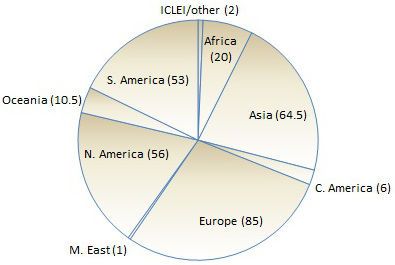
\includegraphics[width=\textwidth]{Fig01.jpg}}
\captionof{figure}{Community gardens in the north of Lisbon (Portugal). \label{Fig01}}
\end{minipage}




\end{multicols}
\vspace{\baselineskip}

\setlength{\tabcolsep}{3pt}
\noindent
\begin{footnotesize}
\begin{minipage}{\columnwidth}\centering
\captionof{table}{Results of a General Linear Model for the proportion of agricultural land under organic farming in French Departments (2008) as a function of plant biodiversity, landscape connectivity, proportion of Natura 2000 protected areas, latitude, longitude, altitude, human population size and department area. The number of data points is 95, the adjusted R$^2$ of the model 0.50, and the intercept 1.457 (s.e. = 2.074).}
\label{Tab01}
\begin{tabular}{lrrrrrrrr}
\toprule
 & N of plant taxa & Landscape connectivity & \% Natura 2000 & Latitude & Longitude & Altitude & Human population & Area \\
\midrule
parameter estimate & 0.264 & 0.047 & 0.113 & -0.084 & 0.003 & 0.038 & 0.056 & 0.327 \\
s.e. & 0.486 & 0.101 & 0.09 & 0.024 & 0.017 & 0.172 & 0.132 & 0.139 \\
\textit{P}-value & 0.59 & 0.64 & 0.21 &\textbf{ \textless0.001} & 0.87 & 0.82 & 0.67 & \textbf{0.02}\\
\bottomrule
\end{tabular}
\end{minipage}

\end{footnotesize}

\vspace{\baselineskip}
\begin{multicols}{2}


\begin{enumerate}[label=\alph*)]
\item
\end{enumerate}